\documentclass[tikz,border=5pt]{standalone}
\usepackage[utf8]{inputenc}
\usetikzlibrary{shapes.geometric, arrows, positioning}

\tikzstyle{startstop} = [rectangle, rounded corners, minimum width=3cm, minimum height=1cm,text centered, draw=black, fill=violet!30]
\tikzstyle{question} = [rectangle, rounded corners, minimum width=3cm, minimum height=1cm,text centered, draw=black, fill=blue!30]
\tikzstyle{analysis} = [rectangle, minimum width=3cm, minimum height=1cm,text centered, draw=black, fill=green!30]
\tikzstyle{result} = [rectangle, minimum width=3cm, minimum height=1cm,text centered, draw=black, fill=yellow!30]
\tikzstyle{arrow} = [thick,->,>=stealth]

\begin{document}

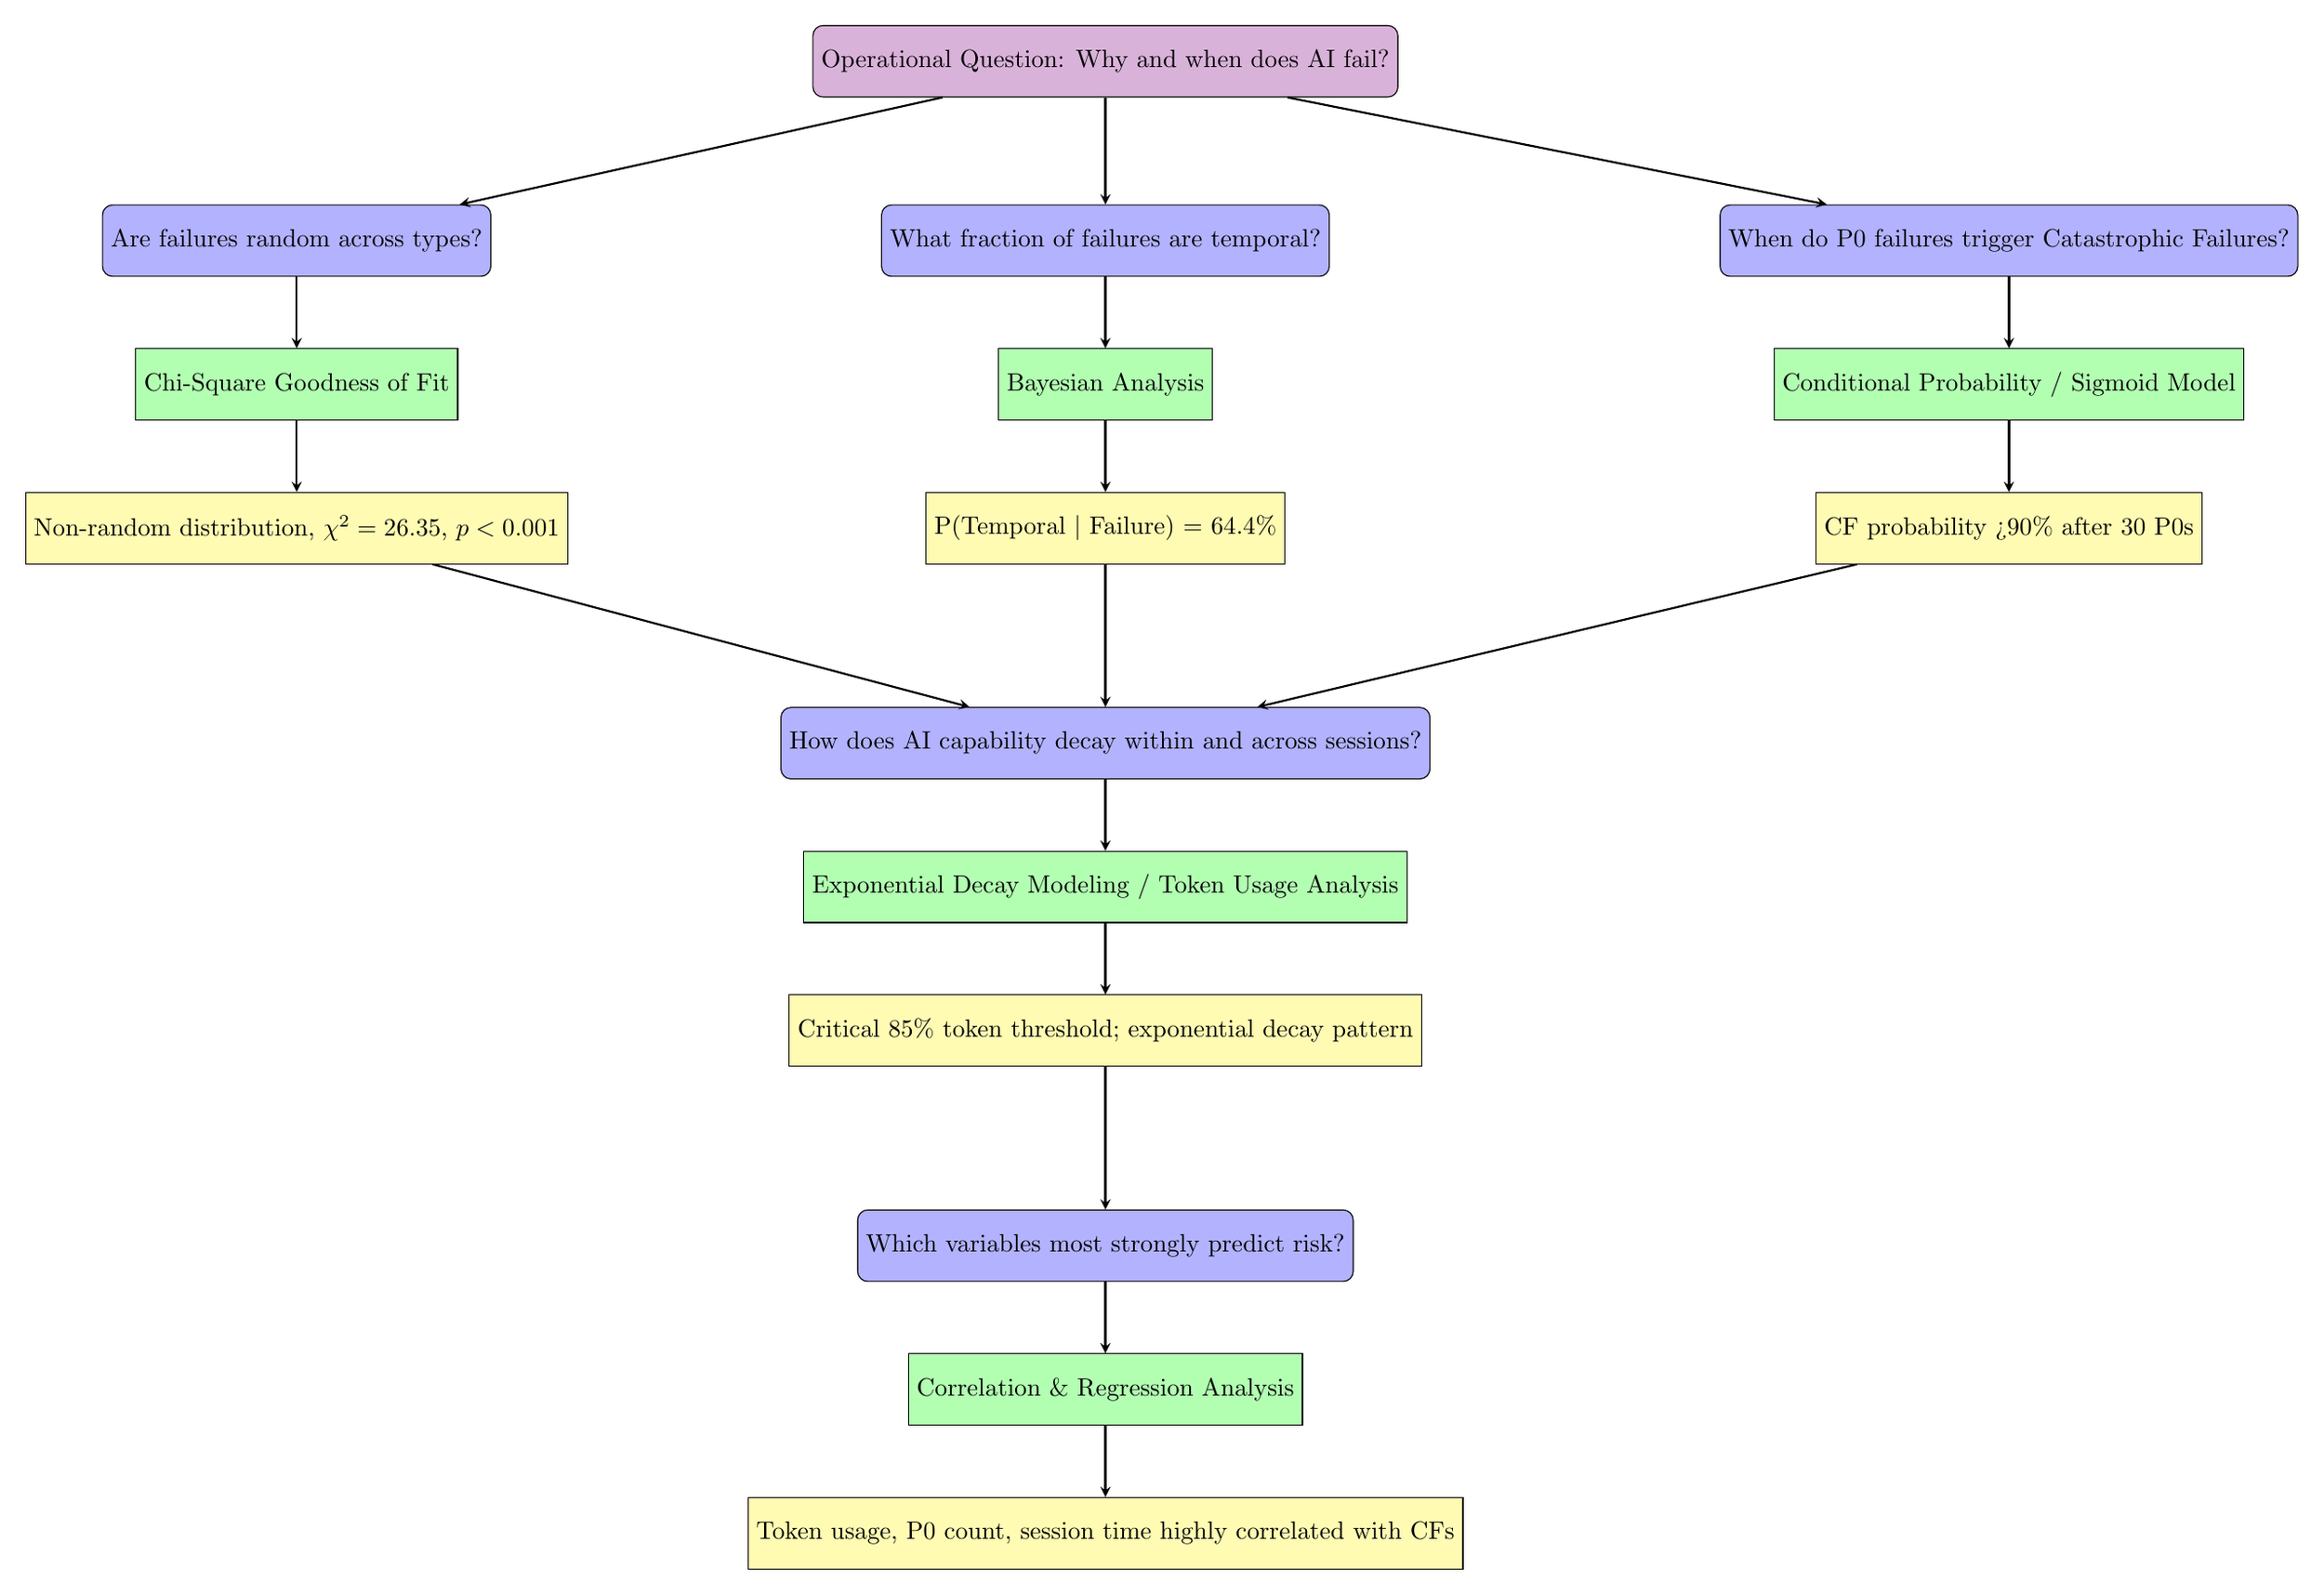
\begin{tikzpicture}[node distance=2cm]

% Nodes
\node (start) [startstop] {Operational Question: Why and when does AI fail?};

\node (q1) [question, below left=1.5cm and 4.5cm of start] {Are failures random across types?};
\node (q2) [question, below=1.5cm of start] {What fraction of failures are temporal?};
\node (q3) [question, below right=1.5cm and 4.5cm of start] {When do P0 failures trigger Catastrophic Failures?};

\node (a1) [analysis, below=1cm of q1] {Chi-Square Goodness of Fit};
\node (a2) [analysis, below=1cm of q2] {Bayesian Analysis};
\node (a3) [analysis, below=1cm of q3] {Conditional Probability / Sigmoid Model};

\node (r1) [result, below=1cm of a1] {Non-random distribution, $\chi^2 = 26.35$, $p < 0.001$};
\node (r2) [result, below=1cm of a2] {P(Temporal $|$ Failure) = 64.4\%};
\node (r3) [result, below=1cm of a3] {CF probability >90\% after 30 P0s};

\node (q4) [question, below=2cm of r2] {How does AI capability decay within and across sessions?};

\node (a4) [analysis, below=1cm of q4] {Exponential Decay Modeling / Token Usage Analysis};

\node (r4) [result, below=1cm of a4] {Critical 85\% token threshold; exponential decay pattern};

\node (q5) [question, below=2cm of r4] {Which variables most strongly predict risk?};

\node (a5) [analysis, below=1cm of q5] {Correlation \& Regression Analysis};

\node (r5) [result, below=1cm of a5] {Token usage, P0 count, session time highly correlated with CFs};

% Arrows
\draw [arrow] (start) -- (q1);
\draw [arrow] (start) -- (q2);
\draw [arrow] (start) -- (q3);

\draw [arrow] (q1) -- (a1);
\draw [arrow] (q2) -- (a2);
\draw [arrow] (q3) -- (a3);

\draw [arrow] (a1) -- (r1);
\draw [arrow] (a2) -- (r2);
\draw [arrow] (a3) -- (r3);

\draw [arrow] (r1) -- (q4);
\draw [arrow] (r2) -- (q4);
\draw [arrow] (r3) -- (q4);

\draw [arrow] (q4) -- (a4);
\draw [arrow] (a4) -- (r4);
\draw [arrow] (r4) -- (q5);
\draw [arrow] (q5) -- (a5);
\draw [arrow] (a5) -- (r5);

\end{tikzpicture}

\end{document}
